\chapter{Metodología y Cronograma de trabajo}
\label{chap:coloso}
\textit{The first chapter introduces fluorescence-based DNA technology and highlights the motivation of the research conducted in the thesis}
\vfill
\minitoc
\newpage

\section{Metodología SCRUM}
\subsection{Visión General}
Scrum es un marco de trabajo en el que equipos cross-funcionales pueden crear productos o desarrollar proyectos de una forma iterativa e incremental. El desarrollo se estructura en ciclos de trabajo llamados Sprints (también conocidos como iteraciones). Estas iteraciones no deben durar más de cuatro semanas cada una (siendo dos semanas la duración más habitual) y tienen lugar una tras otra sin pausa entre ellas. Los Sprints están acotados en el tiempo – finalizan en una fecha determinada independientemente de si el trabajo ha finalizado por completo o no, y jamás se prorrogan. Normalmente los equipos Scrum escogen una duración de Sprint y la mantienen para todos sus Sprints hasta que mejoran y pueden emplear ciclos más cortos. Al principio de cada Sprint, un Equipo cross-funcional (de en torno a siete personas) selecciona elementos (peticiones del cliente) de una lista priorizada. El equipo acuerda un objetivo colectivo respecto a lo que creen que podrán entregar al final del Sprint, algo que sea tangible y que estará “terminado” por completo. Durante el Sprint no se podrán añadir nuevos elementos; Scrum se adapta a los cambios en el siguiente Sprint, pero el pequeño Sprint actual está pensado para concentrarnos en un objetivo pequeño, claro y relativamente estable. Todos los días el Equipo se reúne brevemente para inspeccionar su progreso y ajustar los siguientes pasos necesarios para completar el trabajo pendiente. Al final del Sprint, el Equipo revisa el Sprint con los diferentes Stakeholders (interesados e involucrados en el producto) y realiza una demostración de lo que han desarrollado. Se obtiene feedback que podrá ser incorporado en el siguiente Sprint. Scrum enfatiza un producto “funcionando” al final del Sprint que esté realmente “terminado”. En el caso del software, esto significa un sistema que está integrado, testado, con la documentación de usuario generada y potencialmente entregable.
  \begin{figure}[H]
  	\centering
  	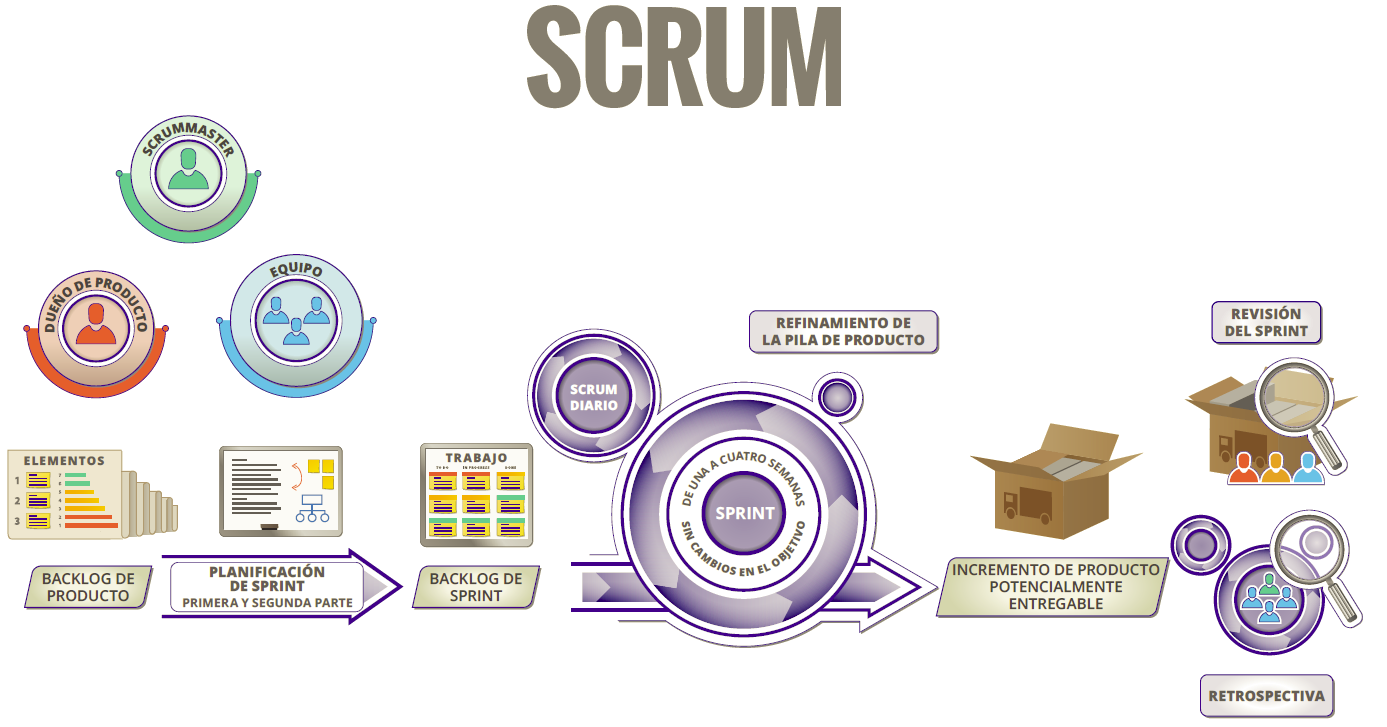
\includegraphics[scale=0.24]{figuras/2a}
  	\captionsetup{width=.95\textwidth}
  	\caption{Visión general de Scrum}
  	\label{figura2a}
  \end{figure}

\subsection{Teoría de Scrum}
Scrum se basa en la teoría de control de procesos empírica o empirismo. El empirismo asegura que el conocimiento procede de la experiencia y de tomar decisiones basándose en lo que se conoce, Scrum emplea un enfoque iterativo e incremental para optimizar la predictibilidad y el control del riesgo. \\

Tres pilares soportan toda la implementación del control de procesos empírico: transparencia, inspección y adaptación. \\

\textbf{Transparencia:} Los aspectos significativos del proceso deben ser visibles para aquellos que son responsables del resultado. La transparencia requiere que dichos aspectos sean definidos por un estándar común, de tal modo que los observadores compartan un entendimiento común de lo que se está viendo.  \\
\textbf{Inspección:} Los usuarios de Scrum deben inspeccionar frecuentemente los artefactos de Scrum y el progreso hacia un objetivo, para detectar variaciones. Su inspección no debe ser tan frecuente como para que interfiera en el trabajo. Las inspecciones son más beneficiosas cuando se realizan de forma diligente por inspectores expertos, en el mismo lugar de trabajo. \\ 
\textbf{Adaptación:} Si un inspector determina que uno o más aspectos de un proceso se desvían de límites aceptables, y que el producto resultante no será aceptable, el proceso o el material que está siendo procesado deben ser ajustados. Dicho ajuste debe realizarse cuanto antes para minimizar desviaciones mayores.  \\

Scrum prescribe cuatro eventos formales, contenidos dentro del Sprint, para la inspección y adaptación y son los siguientes.
  \begin{itemize}
	\item Reunión de Planificación del Sprint (Sprint Planning Meeting)
	\item Scrum Diario (Daily Scrum)
	\item Revisión del Sprint (Sprint Review)
	\item Retrospectiva del Sprint (Sprint Retrospective)
  \end{itemize}
  
  \subsection{Eventos de Scrum}
  En Scrum existen eventos predefinidos con el fin de crear regularidad y minimizar la necesidad de reuniones no definidas en Scrum. Todos los eventos son bloques de tiempo (time-boxes), de tal modo que todos tienen una duración máxima. Una vez que comienza un Sprint, su duración es fija y no puede acortarse o alargarse. Los demás eventos pueden terminar siempre que se alcance el objetivo del evento, asegurando que se emplee una cantidad apropiada de tiempo sin permitir desperdicio en el proceso. \\
  
  Además del propio Sprint, que es un contenedor del resto de eventos, cada uno de los eventos de Scrum constituye una oportunidad formal para la inspección y adaptación de algún aspecto. Estos eventos están diseñados específicamente para habilitar las vitales transparencia e inspección. La falta de alguno de estos eventos da como resultado una reducción de la transparencia y constituye una oportunidad perdida para inspeccionar y adaptarse.
  
  \subsubsection{El Sprint}
  El corazón de Scrum es el Sprint, es un bloque de tiempo (time-box) de un mes o menos durante el cual se crea un incremento de producto “Terminado”, utilizable y potencialmente desplegable. Es más conveniente si la duración de los Sprints es consistente a lo largo del esfuerzo de desarrollo. Cada nuevo Sprint comienza inmediatamente después de la finalización del Sprint previo.
  
  \subsubsection{Revisión de Sprint}
  Al final del Sprint se lleva a cabo una Revisión de Sprint para inspeccionar el Incremento y adaptar la Lista de Producto si fuese necesario. Durante la Revisión de Sprint, el Equipo Scrum y los interesados colaboran acerca de lo que se hizo durante el Sprint. Basándose en esto, y en cualquier cambio a la Lista de Producto durante el Sprint.
  
  \subsubsection{Retrospectiva de Sprint}
  La Retrospectiva de Sprint es una oportunidad para el Equipo Scrum de inspeccionarse a sí mismo y crear un plan de mejoras que sean abordadas durante el siguiente Sprint. La Retrospectiva de Sprint tiene lugar después de la Revisión de Sprint y antes de la siguiente Reunión de Planificación de Sprint. Se trata de una reunión restringida a un bloque de tiempo de tres horas para Sprints de un mes.
  
  \subsection{El equipo Scrum}
  El Equipo Scrum consiste en un Dueño de Producto (Product Owner), el Equipo de Desarrollo (Development Team) y un Scrum Master. Los Equipos Scrum son autoorganizados y multifuncionales. El modelo de equipo en Scrum está diseñado para optimizar la flexibilidad, la creatividad y la productividad. \\
  
  Los Equipos Scrum entregan productos de forma iterativa e incremental, maximizando las oportunidades de obtener retroalimentación. Las entregas incrementales de producto terminado aseguran que siempre estará disponible una versión potencialmente útil y funcional del producto. 
  
  \subsubsection{El Dueño de Producto}
  El Dueño de Producto es el responsable de maximizar el valor del producto y del trabajo del Equipo de Desarrollo. El cómo se lleva a cabo esto podría variar ampliamente entre distintas organizaciones, Equipos Scrum e individuos.
  
  \subsubsection{El Equipo de Desarrollo}
  El Equipo de Desarrollo consiste en los profesionales que desempeñan el trabajo de entregar un Incremento de producto terminado, que potencialmente se pueda poner en producción, al final de cada Sprint. Solo los miembros del Equipo de Desarrollo participan en la creación del Incremento. Los Equipos de Desarrollo son estructurados y empoderados por la organización para organizar y gestionar su propio trabajo. La sinergia resultante optimiza la eficiencia y efectividad del Equipo de Desarrollo.
  
  \subsubsection{El Scrum Master}
  El Scrum Master es el responsable de asegurar que Scrum es entendido y adoptado. Los Scrum Masters hacen esto asegurándose de que el Equipo Scrum trabaja ajustándose a la teoría, prácticas y reglas de Scrum. El Scrum Master es un líder que está al servicio del Equipo Scrum. El Scrum Master ayuda a las personas externas al Equipo Scrum a entender qué interacciones con el Equipo Scrum pueden ser de ayuda y cuáles no. El Scrum Master ayuda a todos a modificar estas interacciones para maximizar el valor creado por el Equipo Scrum.

\section{Cronograma}
  \begin{figure}[H]
  	\centering
  	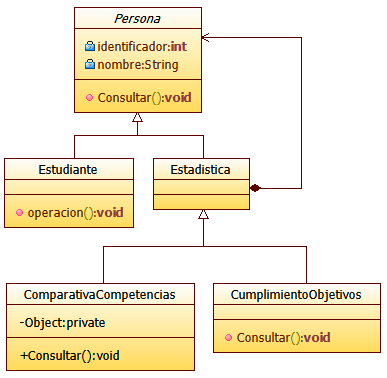
\includegraphics[scale=0.8]{figuras/3}
  	\captionsetup{width=.95\textwidth}
  	\caption{Cronograma}
  	\label{figura3}
  \end{figure}

\chapter{Arquitectura Empresarial}
\label{chap:aEmpresarial}
\textit{The first chapter introduces fluorescence-based DNA technology and highlights the motivation of the research conducted in the thesis}
\vfill
\minitoc
\newpage

\section{Arquitectura empresarial}
La definición de arquitectura empresarial surge frente a la necesidad de alinear las tecnologías de información a los objetivos estratégicos del negocio. Algunas definiciones de arquitectura empresarial se presentan a continuación:
  
  \begin{itemize}
	\item \textit{IEEE Std. 1471-2000:} \\
	“…organización fundamental de un sistema, compuesta por sus componentes, las relaciones entre ellos y su ambiente y los principios que gobiernan su diseño y evolución”.
	\item \textit{The Open Group Architecture Framework:} \\
	“… la arquitectura empresarial se puede definir de dos posibles formas dependiendo del contexto en que se utilice 1) una descripción formal de un sistema o un plan detallado de un sistema a nivel de sus componentes para guiar su implementación; o 2) una estructura de componentes, sus interrelaciones, y los principios y guías que gobiernan su diseño y evolución en el tiempo”.
	\item \textit{International Enterprise Architecture Institute:} \\
	“El análisis y documentación de una organización en su estado actual y futuro desde las perspectivas de negocio, tecnología y estrategias integradas”.
	\item \textit{Federal Enterprise Architecture Framework, 1ra versión – 1999:}
	“… las arquitecturas empresariales son modelos que se aplican de manera sistemática y completa para definir el ámbito presente o futuro de una organización. Arquitecturas empresariales son esenciales para la evolución y desarrollo de nuevos sistemas de información que optimicen el valor de la misión de una organización…”
	\item \textit{Gartner Research:} \\
	“Una arquitectura empresarial es un proceso de planeamiento estratégico que traduce la visión y estrategias de negocio de una organización en un efectivo plan de cambio empresarial”.
  \end{itemize}

  En conclusión arquitectura empresarial es alinear los objetivos estratégicos de una organización con tecnología, describiendo el estado actual de la organización y proyectándonos a una visión futura con la implementación de nuevas tecnologías.
  
\section{Componentes de una Arquitectura Empresarial}
Los diferentes framework de arquitectura empresarial realizan un planteamiento de los componentes o dominios de arquitectura que son los elementos que definen el funcionamiento de una empresa. En la figura 1.5 se presentan los componentes de arquitectura empresarial: Arquitectura de negocio, arquitectura de información, arquitectura de sistemas de información y arquitectura tecnológica.
  
  \begin{figure}[H]
  	\centering
  	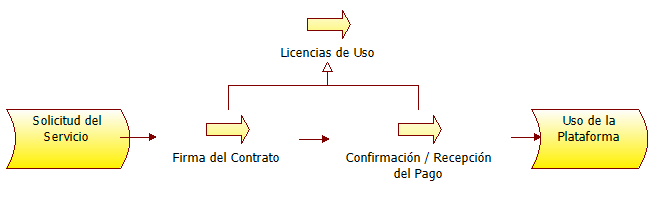
\includegraphics[scale=0.5]{figuras/4}
   	\captionsetup{width=.95\textwidth}
   	\caption{Componentes de Arquitectura Empresarial}
   	\label{figura4}
  \end{figure}
  
  \subsection{Arquitectura de negocio}
  Para Ralph Whittle, “La primera vista representa la arquitectura de negocio, la cual se encarga de la descripción de la estructura organizacional, de los procesos de negocio, los sistemas de planeación y control, los mecanismos de gobierno y administración de políticas y procedimientos en el entorno empresarial. Esta vista de arquitectura es la que refleja el valor del negocio obtenido de las sinergias y resultados que se producen desde las otras vistas de arquitectura que le preceden. La arquitectura de negocio recibe como insumo principal el plan estratégico de la empresa, los lineamientos corporativos, los indicadores de gestión, y se nutre de la misión, la visión, las estrategias y los objetivos corporativos. Las estrategias y objetivos de alto nivel los traducen en requerimientos que son relevantes para el negocio”.
  \subsection{Arquitectura de información}
  Para Richard Wurman, “La segunda vista representa la arquitectura de información, la cual describe los activos lógicos y físicos de los datos como un activo de la empresa, y la administración de los recursos de información; esta perspectiva muestra cómo los recursos de información están siendo administrados, compartidos y utilizados por la organización. \\
  La arquitectura de información es una disciplina que organiza conjuntos de información, permitiendo que cualquier persona los entienda y los integre a su propio conocimiento de manera simple. La construcción de una arquitectura de información requiere el levantamiento de un inventario de los objetos de negocio que representan los activos de información que están disponibles y que son utilizados por la organización. La información juega un rol fundamental para el funcionamiento de los sistemas de información y de los proceso de negocio”
  \subsection{Arquitectura de sistemas de información o aplicaciones}
  Para Richard Wurman, “La tercera vista representa la Arquitectura de sistemas de información que incorpora soluciones aplicativas que apoyan al negocio basadas en las capacidades funcionales requeridas y las estrategias de tecnología definidas, e identifica componentes y servicios que den respuesta a necesidades comunes de las áreas de negocio. La arquitectura aplicativa define qué clase de aplicaciones son relevantes para la empresa y lo que estas aplicaciones necesitan para gestionar los datos y presentar la información”.
  \subsection{Arquitectura tecnológica}
  Según Jaap Schekkerman, “La arquitectura técnica define la estrategia y arquitectura tecnológica en la infraestructura de TI, y el marco tecnológico de las plataformas computacionales y bases de datos que deben soportar las distintas soluciones del negocio, así como los mecanismos de almacenamiento de los datos e información, las redes de datos, los centros de procesamiento de datos y los servicios integrados de tecnología”.
 
\chapter{Framework y Modelado}
\label{chap:Archimate}
\textit{The first chapter introduces fluorescence-based DNA technology and highlights the motivation of the research conducted in the thesis}
\vfill
\minitoc
\newpage

\section{The Open Group}
The Open Group es un consorcio de la industria del software que provee estándares abiertos neutrales para la infraestructura de la informática. Fue formado a partir de la fusión de X/Open con OSF en 1996. The Open Group es muy famoso por sus sistemas de certificación de la marca UNIX; en el pasado el grupo fue reconocido por publicar el artículo Single UNIX Specification, el cual extiende los estándares de POSIX y es la definición oficial del sistema operativo conocido como UNIX. Sus miembros incluyen un conjunto de empresas y agencias gubernamentales, como por ejemplo Capgemini, Fujitsu, Hitachi, HP, IBM, NEC, Departamento de Defensa de Estados Unidos, NASA y otros.

\section{TOGAF}
TOGAF es un marco de referencia de arquitectura. En términos simples, TOGAF es una herramienta para asistir en la aceptación, creación, uso, y mantenimiento de arquitecturas. Está basado en un modelo iterativo de procesos apoyado por las mejores prácticas y un conjunto reutilizable de activos arquitectónicos existentes. \\

TOGAF es desarrollado y mantenido por el Foro de Arquitectura de The Open Group. La primera versión de TOGAF, desarrollada en 1995, se basó en el Marco de Referencia de Arquitectura Técnica para la Gestión de la Información del Ministerio de Defensa Estadounidense (TAFIM por sus siglas en inglés). Comenzando con esta solida fundación, el Foro de Arquitectura de The Open Group ha desarrollado versiones sucesivas de TOGAF con regularidad y ha publicado cada una en el sitio web público de The Open Group. \\

Según The Open Group, el 80\% de las grandes organizaciones a nivel mundial ha adoptado TOGAF como marco de referencia para sus Arquitecturas Empresariales; así mismo, decenas de miles de personas en todo el mundo han recibido formación y certificación en el marco del programa 'Open CA'.

Por otro lado, TOGAF se basa en modelos descriptivos que permiten definir la arquitectura desde diversos y estratégicos puntos de vista, para establecer a nivel general las necesidades, limitaciones y oportunidades del negocio.

  \subsection{¿Qué es Arquitectura para TOGAF?}
  Uno de los conceptos clave para cualquier proceso de arquitectura empresarial es la comprensión misma de la Arquitectura, ya que ésta determina, en parte, el enfoque desde el cual se adoptará el modelo. En TOGAF, “Arquitectura” tiene dos significados según el contexto:
  \begin{enumerate}
  	\item Una descripción formal de un sistema o un plano detallado del sistema al nivel de sus componentes para orientar su implementación.
  	\item La estructura de componentes, sus interrelaciones y los principios y guías que gobiernan su diseño y evolución a través del tiempo.
  \end{enumerate}
  
  \subsection{Arquitectura soportada por TOGAF}
  TOGAF cubre el desarrollo de cuatro tipos relacionados en la arquitectura. Estos cuatro tipos de arquitectura son comúnmente aceptados como subconjuntos de una arquitectura empresarial, los cuales TOGAF esta diseñado para soportar.
  
    \begin{table}[H]
    	\centering
    	\begin{tabular}{lp{8cm}}
    		\toprule
    		\textbf{Tipo de Arquitectura} & \textbf{Descripción} \\
    		\midrule
    		\textbf{Arquitectura de Negocio} & La estrategia de negocio, gobierno, organización y procesos clave de la organización. \\
    		\textbf{Arquitectura de datos} & La estructura de datos lógicos y fisicos que posee una organización y sus recursos de gestión de datos. \\
    		\textbf{Arquitectura de aplicación} & Un plano (blueprint en inglés) de las aplicaciones individuales a implementar, sus interacciones y sus relaciones con los procesos de negocio principales de la organización.
    		 \\
    		\textbf{Arquitectura tecnológica} & Las capacidades de software y hardware que se requieren para apoyar la implementación de servicios de negocio, datos y aplicación. Esto incluye infraestructura de IT, capa de mediación (middleware en ingles), redes, comunicaciones, procesamiento y estándares.
    		\\
    		\bottomrule
    	\end{tabular}
    	\captionsetup{width=.95\textwidth}
    	\caption{Tipos de la arquitectura soportados por TOGAF}
    	\label{tabla1} 
    \end{table}
    
  \subsection{Método de desarrollo de la Arquitectura (ADM)}
  El \textbf{ADM} describe cómo obtener una Arquitectura Empresarial que sea especifica para la organización y para responder a los requerimientos del negocio. El ADM es el componente principal de TOGAF y proporciona dirección a los arquitectos en varios niveles:
  \begin{itemize}
  	\item Proporciona varias fases de desarrollo de arquitectura (Arquitectura de Negocio, Arquitecturas de Sistemas de Información, Arquitectura Tecnológica) en un ciclo, que sirve como una plantilla general de procesos para la actividad de desarrollo de la arquitectura.
  	\item Proporciona una narrativa de cada fase de la arquitectura, describiendo la fase en términos de objetivos, enfoque, entradas, pasos a seguir, y salidas. Las secciones de entradas y salidas proporcionan una definición de la estructura del contenido de arquitectura y entregables (una descripción detallada de las entradas de la fase y las salidas de la fase se da en el Marco de Referencia del Contenido Arquitectónico).
  	\item Proporciona resúmenes multi-fase que abordan también la Gestión de Requerimientos.
  \end{itemize}
  
  El ADM es el resultado de las contribuciones de numerosos profesionales de la arquitectura y constituye el núcleo de TOGAF. Es un método para obtener Arquitecturas Empresariales que son específicas para la organización, y está especialmente diseñado para responder a los requerimientos del negocio. El ADM describe:
  
  \begin{itemize}
  	\item Un modo confiable y probado para desarrollar y utilizar una Arquitectura Empresarial
  	\item Un método para desarrollar arquitecturas en diferentes niveles1 (negocio, aplicaciones, datos, tecnología) que permiten al arquitecto asegurar que un conjunto complejo de requerimientos se aborden adecuadamente
  	\item Un conjunto de guías y técnicas para el desarrollo de arquitectura
 \end{itemize}
  
  \subsubsection{Fases del ADM}
  El ADM consiste en varias Fases que se desplazan cíclicamente a través de una serie de Dominios de Arquitectura y permiten al arquitecto asegurar que un conjunto complejo de requerimientos se aborden adecuadamente. La estructura básica del ADM se muestra en la Figura 2.
  
    \begin{figure}[H]
    	\centering
    	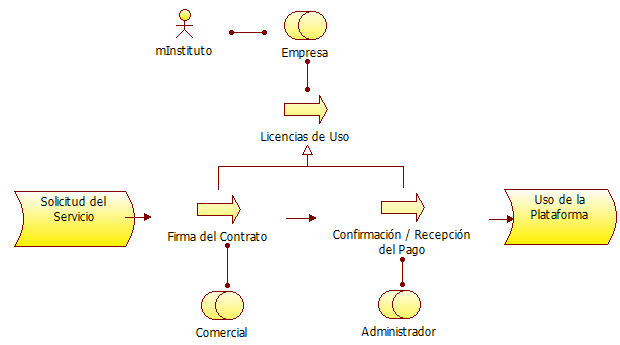
\includegraphics[scale=0.5]{figuras/5}
    	\captionsetup{width=.95\textwidth}
    	\caption{El ciclo del Modelo de Desarrollo de la Arquitectura}
    	\label{figura5}
    \end{figure}
    
    El ADM se aplica iterativamente durante todo el proceso, entre las diferentes Fases, y dentro de ellas. Durante todo el ciclo del ADM se debe realizar una validación frecuente de los resultados respecto a los requerimientos originales, tanto aquellos del ciclo completo del ADM como los de la Fase particular del proceso. Esta validación debe reconsiderar el alcance, los detalles, el plan y los hitos. Cada Fase debe considerar los activos producidos a partir de las iteraciones anteriores del proceso y los activos externos de mercado, así como otros marcos de referencia o modelos. \\
    
    El ADM apoya el concepto de iteración en tres niveles:
    \begin{itemize}
    	\item \textbf{Ciclo alrededor del ADM:} El ADM se presenta de manera circular indicando que la finalización de una Fase de trabajo en la arquitectura alimenta directamente las Fases subsecuentes de trabajo en la arquitectura.
    	\item \textbf{Iteración entre Fases:} TOGAF describe el concepto de la iteración a través de Fases (por ejemplo, volviendo a la Arquitectura de Negocio posteriormente a la finalización de la Arquitectura Tecnológica).
    	\item \textbf{Ciclo alrededor de una Fase individual:} TOGAF apoya la ejecución repetida de las actividades dentro de una Fase individual del ADM como una técnica para elaborar contenido arquitectónico.
   \end{itemize}
   
   \begin{table}[H]
   	\centering
   	\begin{tabular}{|p{4cm}|p{10cm}|}
   		\toprule
   		\textbf{Fase de ADM} & \textbf{Actividad} \\
   		\midrule
   		\textbf{Gestión de Requerimientos} & Cada etapa de un proyecto de TOGAF está basada en los requerimientos del negocio, incluyendo su validación.
   		Los requerimientos se identifican, se almacenan y se gestionan al ingreso y egreso de las fases relevantes del ADM, las cuales eliminan, abordan, y priorizan los requerimientos. \\ \hline
   		\textbf{A. Visión de arquitectura} & Establece el alcance, las limitaciones y expectativas de un proyecto de TOGAF. Crea la Visión de la Arquitectura. Identifica a los Interesados. Valida el contexto de negocio y crea la Declaración de Trabajo de Arquitectura. Obtiene aprobaciones. \\ \hline
   		\textbf{B. Arquitectura de Negocio C. Arquitecturas de sistemas de información D. Arquitectura tecnológica} & Desarrolla arquitecturas en cuatro dominios:
   		    \begin{enumerate}
   		    	\item Negocio
   		    	\item Sistemas de Información - Aplicaciones
   		    	\item Sistemas de Información - Datos
   		    	\item Tecnología
   		    \end{enumerate}
   		En cada caso, desarrolla la Arquitectura de la línea de base y de destino y analiza las brechas entre ambas. \\  \hline
   		\textbf{E. Oportunidades y soluciones} & Realiza la planificación de la implementación inicial y la identificación de medios de entrega para los Bloques de Construcción identificados en las Fases anteriores. Determina si se requiere un enfoque incremental, y si asi fuera, identifica las Arquitecturas de Transición. \\ \hline
   		\textbf{F. Planificación de la migración} & Desarrolla el Plan detallado de Implementación y Migración que aborda cómo moverse de la Arquitectura de la Linea de Base a la Arquitectura de Destino. \\ \hline
   		\textbf{G. Gobierno de la Implementación} & Proporciona supervisión arquitectónica para la implementación. Prepara y publica Contratos de Arquitectura. Asegura que el proyecto de implementación esté en conformidad con la arquitectura. \\ \hline
   		\textbf{H. Gestión de cambios de la Arquitectura} & Proporciona seguimiento continuo y un proceso de gestión de cambios para asegurar que la arquitectura responda a las necesidades de la empresa y que se maximice el valor de la arquitectura para el negocio. \\
   		\bottomrule
   	\end{tabular}
   	\captionsetup{width=.95\textwidth}
   	\caption{Actividades del Método de Desarrollo de la arquitectura por Fase}
   	\label{tabla2} 
  \end{table}

\section{Archimate 2.1}
ArchiMate nace como un lenguaje de modelado de arquitecturas empresariales el cual tiene como objetivo proveer una representación uniforme de los diagramas que describen la arquitectura empresarial de una organización, permitiendo comprender las diferentes áreas o capas empresariales: estrategia, negocio, información, aplicaciones e infraestructura tecnológica; describiendo los diferentes dominios, relaciones, dependencias e incorporando el concepto de orientación a servicios. \\

El principal elemento en esta metodología es el servicio, que está definido como una unidad de funcionalidad que un actor (sistema o una organización) pone a disposición del ambiente de trabajo. Se adopta otro concepto ya existente: el concepto de arquitectura en capas. En una arquitectura orientada a servicios, cada capa proporciona servicios que pueden ser consumidos por capas de nivel superior, y cada capa utiliza los servicios proporcionados por capas de nivel inferior. \\
  
  \subsection{Versiones}
  Desde el año 2008 que la propiedad y los derechos de la arquitectura ArchiMate fueron transferidos al Open Group, por parte del consorcio de Universidades, empresas y el Gobierno holandés, se han publicado tres versiones de la arquitectura: ArchiMate 1.0, lanzada el año 2008 como un estándar técnico; ArchiMate 2.0, lanzada el año 2012 como un estándar; ArchiMate 2.1, en el año 2013, constituye la última versión lanzada como actualización a la versión 2.0, donde se considerando comentarios de la comunidad que aplicaban el estándar. \\
  
  La primera versión, ArchiMate 1.0, fue considerada como ya un estándar formal técnico teniendo como base lo realizado por el equipo de desarrollo del estándar. Cabe recalcar que este equipo tomó como referencia a otro estándar el de la IEEE 1471, el mismo que es utilizado para describir el diseño de una arquitectura de software. Este estándar técnico describe ArchiMate como un lenguaje que complementa al marco de trabajo (framework) TOGAF, proporcionado un juego de conceptos y definiciones que permiten representar a través de un leguaje unificado y de representación gráfica un diseño de arquitectura empresarial basado en el framework TOGAF. Se plantea el lenguaje ArchiMate como una correspodencia a las principales vistas que son definidas en la arquitectura TOGAF ADM (ADM - Architecture Develppment Method), específicamente no se hace uso de todas las vistas que menciona TOGAF, como se ilustra en la Figura 1, estás son alineadas a las tres capas que establece el estándar ArchiMarte: Business, Application, Technology. La no coincidencia de todas las capas de ArchiMate con TOGAF denota que el lenguaje está basado en el framework, el cual sí amplia y considera aspectos mucho más profundos concernientes a la arquitectura empresarial, decisiones estratégicas y de dirección. ArchiMate ofrece más un estándar formal donde se aterrizan en un diseño y un lenguaje esquemas donde se permite desarrollar la arquitectura empresarial del cual se derivarán procedimientos más operativos. \\
  
  ArchiMate 2.0, es lanzada en el año 2012 oficialmente como un estándar que conserva gran parte de su versión anterior (1.0) pero en esta ya se incluyen retroalimentaciones por parte de los usuarios del estándar, agregando así nuevas características. Esta nueva versión aparecen dos extensiones: Motivación, e Implementación y Migración. La primera considera aspectos de modelamiento de los interesados, manejos de cambios, objetivos del negocio, principios y requerimientos, se alinea principalmente a la fase inicial de las vistas de TOGAF. La extensión de Implementación y Migración, está diseñada para el manejo del portafolio del proyecto, análisis de brecha, transiciones y planes de migración, principalmente está enfocada a las fases finales de TOGAF. Ambas extensiones incluyen nuevos conceptos que dan atención a las inquietudes y experiencias de los practicantes del estándar en su versión anterior. Así tenemos los conceptos de Ubicación, que brinda un punto de vista conceptual que puede ser asignado a los elementos estructurales e indirectamente también determina sus comportamientos; y la de Función de Infraestructura, que modela el comportamiento interno de un nodo dentro de la capa de tecnología, esto permite mejorar la consistencia de la capa de tecnología con las otras dos capas (Negocios y Aplicación). \\
  
  La más reciente versión de ArchiMate es la 2.1, lanzada el año 2013, esta conserva la gran mayoría de características de su versión anterior (2.0), el motivo de su actualización se debe al direccionamiento de los comentarios de los usuarios que por años han venido usando haciendo que los mismos sean considerados y han constituido de aportes para brindar de mayores detalles y aclaraciones a los aspectos definidos por el estándar.
  
 \begin{figure}[H]
   	\centering
   	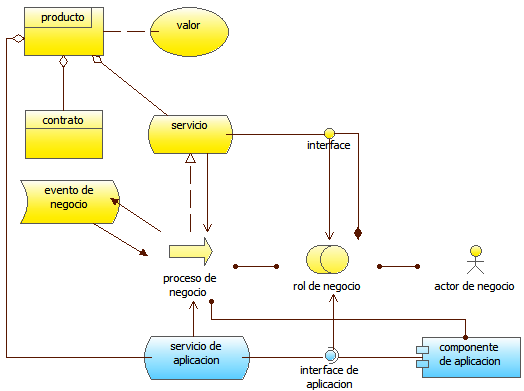
\includegraphics[scale=0.3]{figuras/6}
   	\captionsetup{width=.95\textwidth}
   	\caption{Metamodelos y diferentes niveles de especificación}
   	\label{figura6}
 \end{figure}
  
  \subsection{Conceptos centrales}
  El lenguaje central consiste de tres tipos de elementos:
    \begin{itemize}
	  \item \textbf{Elementos de estructura activa:} Es una entidad capaz de ejercer comportamientos, tales como los actores del negocio, componentes de aplicación
	  \item \textbf{Elementos de comportamiento:} Es una unidad de actividad ejecutada por uno o más elementos de estructura activa.
	  \item \textbf{Elementos de estructura pasiva:} Es un objeto sobre el cual se ejecuta un comportamiento.
	  \item \textbf{Servicio:} Es una unidad de funcionalidad que el sistema provee
	  \item \textbf{Interfaz:} Es el punto de acceso donde uno o más servicios son hechos disponibles al entorno. Provee una vista externa sobre el proveedor de servicio y oculta su estructura interna.
	  \item Para nombrar los roles de las interrelaciones, se utiliza una convención similar a la de UML(pero usando verbos en lugar de sustantivos).
	  \item Si no se muestra cardinalidad alguna al final de un interrelación, se asume una 0..* (cero o más).
    \end{itemize}
  Estos elementos tienen como inspiración el lenguaje natural donde una sentencia tiene un sujeto (estructura activa), un verbo (comportamiento) y un predicado (estructura pasiva)
  
     \begin{figure}[H]
     	\centering
     	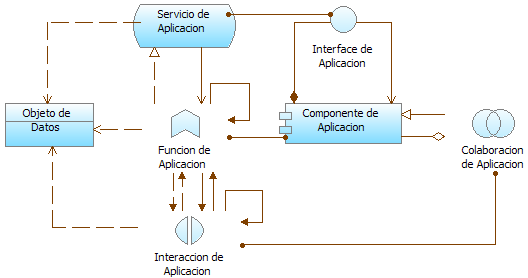
\includegraphics{figuras/7}
     	\captionsetup{width=.95\textwidth}
     	\caption{Conceptos básicos de ArchiMate}
     	\label{figura7}
     \end{figure}
  
  \subsection{Colaboración e interacción}
  Si vamos a un nivel más profundo en la estructura del lenguaje, se distingue entre el comportamiento que es realizado por un elemento de estructura única (Ejemplo: actor, rol, componentes, etc.), o comportamiento colectivo (Interacción) que se realiza por una colaboración de varios elementos de la estructura.
  
  \begin{itemize}
  	\item \textbf{Colaboración:} Es una (temporal) agrupación (o agregación) de dos o más elementos de estructura, trabajando juntos para realizar algún comportamiento colectivo. Este comportamiento colectivo puede ser modelado como una interacción.
  	\item \textbf{Interacción:} Es una unidad de comportamiento llevada a cabo por una colaboración de dos o más elementos de estructura.
  \end{itemize}
 
  \begin{figure}[H]
   	\centering
   	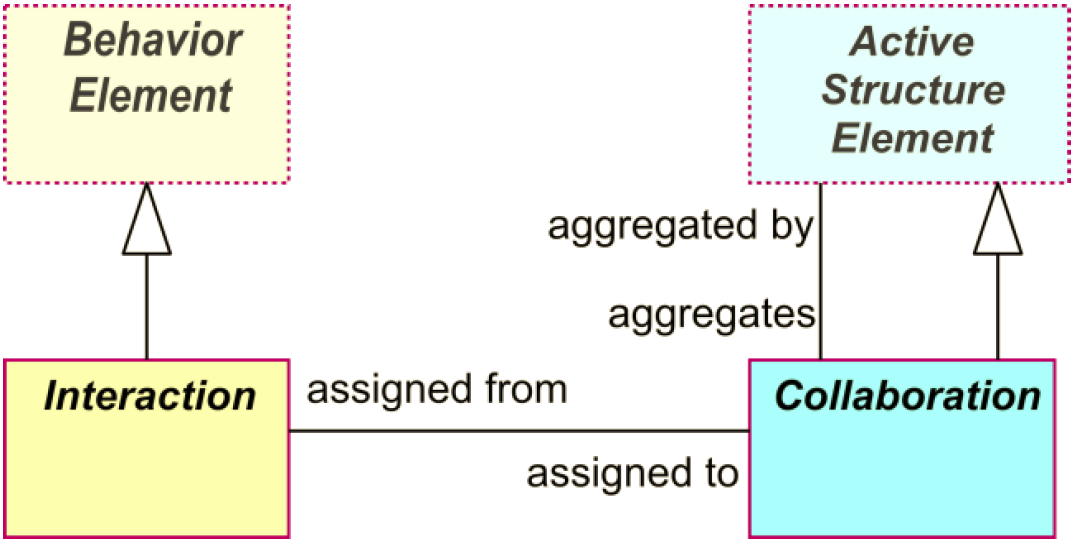
\includegraphics[scale=0.25]{figuras/8}
   	\captionsetup{width=.95\textwidth}
   	\caption{Colaboración e interacción}
   	\label{figura8}
  \end{figure}
  
  \subsection{Relaciones}
  Al lado de los conceptos fundamentales antes reseñadas, ArchiMate contiene un conjunto básico de las relaciones. Varias de estas relaciones han sido adoptadas a partir de conceptos de relación correspondientes que se producen en normas existentes. Relaciones tales como la composición, la agregación, asociación y especialización se toman de UML 2.0, mientras que la activación se utiliza en muchos procesos de negocio lenguajes de modelado.
  
  \subsection{Capas}
  En ArchiMate, hay tres diferentes capas para tres niveles diferentes en una arquitectura empresarial: \\
  \begin{itemize}
  	\item \textbf{Capa empresarial.} La capa de negocio ofrece productos y servicios para clientes externos. Estos servicios están implementados internamente por los procesos de negocios y ejecutados por actores de negocio.
  	\item \textbf{Capa de aplicación.} La capa de aplicación es compatible con la capa de negocio por servicios de aplicaciones implementados por software.
  	\item \textbf{Capa de Tecnología.}  La capa de tecnología proporciona los servicios de infraestructura que son necesarios para ejecutar aplicaciones (software). Son implementados por computadores y la comunicación del hardware y software del sistema.
  \end{itemize}
  
  \subsection{Marco de referencia}
Los aspectos y capas identificadas en los apartados anteriores se pueden organizar como un marco de nueve celdas, es importante darse cuenta de que la clasificación de conceptos basados en aspectos y capas es sólo uno y es imposible definir un límite estricto entre los aspecto capas, porque los conceptos que enlazan los diferentes aspectos y capas juegan un papel central en una arquitectura coherente. El trabajo de un arquitecto de la empresa toca varios aspectos, no expresamente contemplados en el marco ArchiMate. Dominios conceptuales, son:
  \begin{itemize}
  	\item Objetivos, principios y requisitos
  	\item Riesgos y seguridad
  	\item Gobierno
  	\item Políticas y reglas de negocio
  	\item Costos
  	\item Rendimiento
  	\item Planificación y evolución
  \end{itemize}
  
  \begin{figure}[H]
   	\centering
   	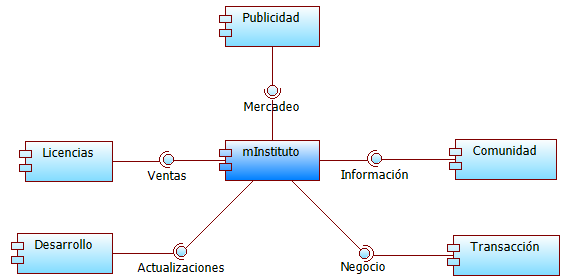
\includegraphics[scale=0.30]{figuras/9}
   	\captionsetup{width=.95\textwidth}
   	\caption{Estructura de la Arquitectura}
   	\label{figura9}
  \end{figure}

  \subsection{Motivación}
  Archimate añade los conceptos de motivación, como objetivo, principio y requisito. Un elemento de motivación se define como un elemento que proporciona el contexto o la razón que está detrás de la arquitectura de la empresa. \\
  
  La gestión de requisitos es una actividad importante en el proceso de diseño y gestión de las arquitecturas empresariales. La metas de las diversas partes interesadas son la base de cualquier cambio en una organización. Estos objetivos deben ser traducidos a los requisitos sobre la arquitectura de la organización. Esta arquitectura debería reflejar cómo los requisitos son realizados por los servicios, procesos y aplicaciones de software en las operaciones del día a día. Por lo tanto, la calidad de la arquitectura está determinada en gran medida por la capacidad de capturar y analizar los objetivos y requisitos pertinentes, el grado en que puede ser realizado por la arquitectura, y la facilidad con que objetivo y los requisitos se puede cambiar. \\
  
  Principios y requerimientos están fuertemente relacionados. Los principios son normas y directrices generales que ayudan a informar y apoyar la forma en que una organización se marca sobre el cumplimiento de su misión. En contraste, las limitaciones de los requisitos dan forma a un diseño específico de la arquitectura empresarial. Esto corresponde a la distinción entre dos interpretaciones generales:
  \begin{itemize}
  	\item Como la estructura de una organización en términos de sus componentes y sus relaciones
  	\item Como un conjunto de principios que se deben aplicar a dicha estructura.
  \end{itemize}
  El alcance de la primera interpretación se refiere a un solo diseño de la organización, mientras que el segundo se refiere a cualquier diseño posible. Los requisitos están asociados con la primera interpretación. En su lugar, los principios son independientes de un diseño específico y tienen que especializarse en las necesidades y en el proceso de diseño de la arquitectura de la organización. \\
  
  La gestión de requisitos inadecuada es una de las principales causas de daños y fallas en los proyectos informáticos, por exceder los presupuestos o plazos, por no entregar los resultados esperados. Por lo tanto, el proceso de gestión de requisitos y el proceso de desarrollo de la arquitectura necesitan estar bien alineados, y la trazabilidad deben mantenerse entre las necesidades de los elementos arquitectónicos que dan cuenta a estos requisitos.
 
  \begin{figure}[H]
   	\centering
   	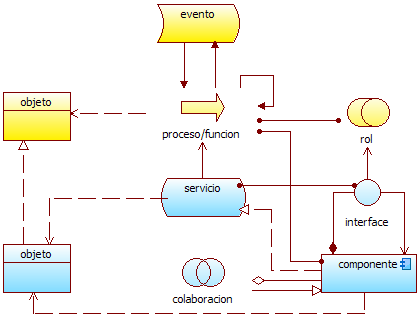
\includegraphics[scale=0.30]{figuras/10}
   	\captionsetup{width=.95\textwidth}
   	\caption{Relación entre los elementos básicos de motivación en ArchiMate}
   	\label{figura10}
  \end{figure}
  
  \subsection{Implementación y Migración}
  La extensión de implantación y migración de ArchiMate añade conceptos para apoyar las fases finales de ADM, relacionados con la implementación y migración de arquitecturas: Fase E (Oportunidades y Soluciones), Fase F (planeamiento de migración), y la Fase G (Gobierno de Aplicación). \\
  
  Esta extensión incluye conceptos para el modelado de los programas y proyectos de aplicación que soportan los programas, el portafolio y la gestión de proyectos. Conceptos que son específicos para uno de estos métodos no son parte de la extensión, pero se pueden definir como la especialización de los conceptos genéricos. De esta manera, el conjunto de conceptos y relaciones que se define en la extensión se mantiene a un mínimo.

  \begin{figure}[H]
  	\centering
   	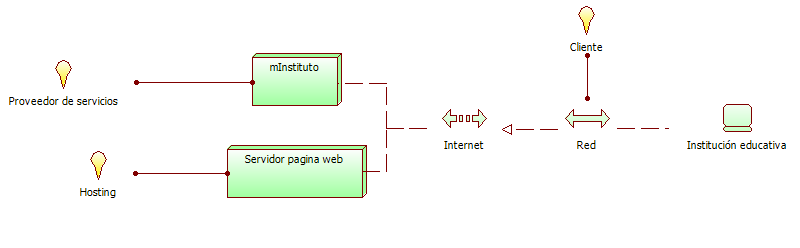
\includegraphics[scale=0.27]{figuras/11}
   	\captionsetup{width=.95\textwidth}
   	\caption{Relaciones entre la motivación, Core, Implementación y Migración}
   	\label{figura11}
  \end{figure}

   \subsection{Archimate: Su relación con TOGAF}
   El lenguaje ArchiMate, tal como se describe en la Norma Técnica, complementa TOGAF, ya que proporciona un conjunto independiente de los proveedores de los conceptos, incluyendo una representación gráfica, que ayuda a crear un modelo integrado coherente "por debajo de la línea de flotación", que puede ser representado en forma de puntos de vista TOGAF. \\
   
   Aunque algunos de los puntos de vista que se definen en TOGAF son difíciles de hacer corresponder con los puntos de vista ArchiMate, el idioma ArchiMate y sus técnicas de análisis sí apoyan los conceptos abordados en estos puntos de vista. Si bien no hay correlación de uno a uno entre ellos, todavía hay una buena cantidad de correspondencia entre los puntos de vista ArchiMate y los puntos de vista que se definen en TOGAF. Aunque los puntos de vista correspondientes de ArchiMate y TOGAF no necesariamente tienen la misma cobertura, podemos ver que muchos puntos de vista de ambos métodos abordan en gran medida los mismos problemas.
   
   TOGAF y ArchiMate pueden ser fácilmente utilizados en conjunto y parecen cubrir gran parte de lo mismo, aunque con algunas diferencias en el alcance y enfoque.
   
     \begin{figure}[H]
     	\centering
     	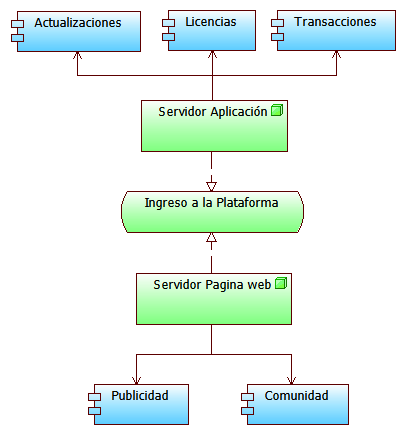
\includegraphics[scale=0.29]{figuras/12}
     	\captionsetup{width=.95\textwidth}
     	\caption{Correspondencia entre ArchiMate (incluyendo extensiones) y TOGAF}
     	\label{figura12}
     \end{figure}

\chapter{Patrones}
\label{chap:patrones}
\textit{The first chapter introduces fluorescence-based DNA technology and highlights the motivation of the research conducted in the thesis}
\vfill
\minitoc
\newpage

\section{Programación Orientada a objetos}
La POO es un paradigma de la programación de computadores; esto hace referencia al conjunto de teorías, estándares, modelos y métodos que permiten organizar el conocimiento, proporcionando un medio bien definido para visualizar el dominio del problema e implementar en un lenguaje de programación la solución a ese problema. \\

La POO se basa en el modelo objeto donde el elemento principal es el objeto, el cual es una unidad que contiene todas sus características y comportamientos en sí misma, lo cual lo hace como un todo independiente pero que se interrelaciona con objetos de su misma clase o de otras clase, como sucede en el mundo real. \\

Una ventaja de la POO frente al paradigma algorítmico es la facilidad que brinda a través de sus herramientas, de concebir, analizar, modelar, diseñar e implementar el mundo real de manera fiel a como se presenta en la realidad; el paso que hay desde la concepción y asimilación del problema hasta la implementación del mismo es un proceso que se hace de manera casi natural. Esto porque el mundo está lleno de objetos reales, los cuales se pueden representar como tales en una solución computarizada.

\section{Patrones de software}
Los patrones para el desarrollo de software son uno de los últimos avances de la Tecnología Orientada a Objetos. Los patrones son una forma literaria para resolver problemas de
ingeniería del software, que tienen sus raíces en los patrones de la arquitectura. \\

Los diseñadores y analistas de software más experimentados aplican de forma intuitiva algunos criterios que solucionan los problemas de manera elegante y efectiva. La ingeniería del
software se enfrenta a problemas variados que hay que identificar para poder utilizar la misma solución (aunque matizada) con problemas similares. \\

El objetivo de los patrones es crear un lenguaje común a una comunidad de desarrolladores para comunicar experiencia sobre los problemas y sus soluciones.

  \subsection{Definiciones}
  Los diferentes autores han dado diversas definiciones de lo que es un patrón software.
  \begin{itemize}
  	\item \textit{Dirk Riehle y Heinz Zullighoven:} \\
  	“Un patrón es la abstracción de una forma concreta que puede repetirse en contextos específicos.”.
 	\item \textit{Richard Gabriel:} \\
  	“  Cada patrón es una regla de tres partes, la cual expresa una relación entre un cierto contexto, un conjunto de fuerzas que ocurren repetidamente en ese contexto y una cierta configuración software que permite a estas fuerzas resolverse por si mismas.”.
  \end{itemize}
  
  \subsection{Clases de patrones software}
  Existen diferentes ámbitos dentro de la ingeniería del software donde se pueden aplicar los patrones:
  \begin{enumerate}
  	\item \textbf{Patrones de Arquitectura:} Expresa una organización o esquema estructural fundamental para sistemas software. Proporciona un conjunto de subsistemas predefinidos, especifica sus responsabilidades, e incluye una guía para organizar las relaciones entre ellos.
  	\item \textbf{Patrones de Diseño:} Proporciona un esquema para refinar los subsistemas o componentes de un sistema software, o las relaciones entre ellos. Describe
  	estructuras repetitivas de comunicar componentes que resuelven un problema de diseño en un contexto particular.
  	\item \textbf{Patrones de Programación:} Un idioma es un patrón de bajo nivel de un lenguaje de programación específico. Describe como implementar aspectos de componentes o de las relaciones entre ellos utilizando las facilidades del lenguaje de programación dado.
  	\item \textbf{Patrones de Análisis:} Describen un conjunto de prácticas que aseguran la obtención de un buen modelo de un problema y su solución.
  	\item \textbf{Patrones Organizacionales:} Describen la estructura y prácticas de las organizaciones.
  \end{enumerate}
  
  \section{Patrones de Diseño}
  Los patrones de diseño tienen un cierto nivel de abstracción. Los patrones de diseño no son
  diseños tales como la realización de listas y tablas hash que pueden ser codificadas en clases y reutilizadas. Un algoritmo puede ser un ejemplo de implementación de un patrón, pero es demasiado incompleto, específico y rígido para ser un patrón. Una regla o heurística puede
  participar en los efectos de un patrón, pero un patrón es mucho más. Los patrones de diseño
  son descripciones de las comunicaciones de objetos y clases que son personalizadas para
  resolver un problema general de diseño en un contexto particular. \\
  
  Un patrón de diseño nombra, abstrae e identifica los aspectos clave de un diseño estructurado, común, que lo hace útil para la creación de diseños orientados a objetos   reutilizables. Los patrones de diseño identifican las clases participantes y las instancias, sus papeles y colaboraciones, y la distribución de responsabilidades. Cada patrón de diseño se
  enfoca sobre un particular diseño orientado a objetos. Se describe cuando se aplica, las características de otros diseños y las consecuencias y ventajas de su uso. \\
  
  Los patrones de diseño se pueden utilizar en cualquier lenguaje de programación orientado a objetos, adaptando los diseños generales a las características de la implementación particular.
  
  \subsection{Clasificación de los patrones de diseño}
  Dado que hay muchos patrones de diseño necesitamos un modo de organizarlos. En esta sección clasificamos los patrones de diseño de tal forma que podamos referirnos a familias de patrones relacionados. La clasificación nos ayuda a saber lo que hace un patrón. Según el libro “Patterns in Java (Volume 1)” existen seis categorías:
  
  \subsubsection{Fundamentales}
  Los patrones de esta categoría son los más fundamentales e importantes patrones de diseño
  conocidos. Estos patrones son utilizados extensivamente en otros patrones de diseño.
  
  \subsubsection{Creación}
  Los patrones de creación muestran la guía de cómo crear objetos cuando sus creaciones requieren tomar decisiones. Estas decisiones normalmente serán resueltas dinámicamente decidiendo que clases instanciar o sobre que objetos un objeto delegará responsabilidades. \\
  
  A menudo hay varios patrones de creación que puedes aplicar en una situación. Algunas  veces se pueden combinar múltiples patrones ventajosamente. En otros casos se debe elegir  entre los patrones que compiten.
  
  \subsubsection{Partición}
  Los patrones de esta categoría proveen la guía sobre como dividir actores complejos y casos de uso en múltiples clases.
  
  \subsubsection{Estructurales}
  Los patrones de esta categoría describen las formas comunes en que diferentes tipos de objetos pueden ser organizados para trabajar unos con otros.
  
  \subsubsection{Comportamiento}
  Los patrones de este tipo son utilizados para organizar, manejar y combinar comportamientos.
  
  \subsubsection{Concurrencia}
  Los patrones de esta categoría permiten coordinar las operaciones concurrentes. Estos patrones se dirigen principalmente a dos tipos diferentes de problemas:
  \begin{enumerate}
  	\item \textbf{Recursos compartidos:}
  	Cuando las operaciones concurrentes acceden a los mismos datos o otros tipos de recursos compartidos, podría darse la posibilidad de que las operaciones interfirieran unas con otras si ellas acceden a los recursos al mismo tiempo. Para garantizar que cada operación se ejecuta correctamente, la operación debe ser protegida para acceder a los recursos compartidos en solitario. Sin embargo, si las operaciones están completamente protegidas, entonces podrían bloquearse y no ser capaces de finalizar su ejecución.
  	\item \textbf{Secuencia de operaciones:}
  	Si las operaciones son protegidas para acceder a un recurso compartido una cada vez, entonces podría ser necesario garantizar que ellas acceden a los recursos compartidos en un orden particular. Por ejemplo, un objeto nunca será borrado de una estructura de datos antes de que esté sea añadido a la estructura de datos.
  \end{enumerate}
  	
  \begin{table}[H]
  	\centering
  	\begin{tabular}{p{7cm}|p{7cm}}
  		\toprule
  		\textbf{Fundamentales} & \textbf{De Creación} \\
  		\midrule
  		\begin{itemize}
  			\item Delegation
  			\item Interface
  			\item Unmitable
  			\item Marker Interface
  			\item Proxy
  		\end{itemize} &
  		\begin{itemize}
  			\item Factory Method
  			\item Abstract Factory
  			\item Builder
  			\item Prototype
  			\item Singleton
  			\item Object Pool
  		\end{itemize} \\
  		\midrule
  		\textbf{De Partición} & \textbf{Estructurales} \\
  		\midrule
  		\begin{itemize}
  			\item Layered Initialization
  			\item Filter
  			\item Composite
  		\end{itemize} &
  		\begin{itemize}
  			\item Adapter
  			\item Iterator
  			\item Bridge
  			\item Facade
  			\item Flyweight
  			\item Dynamic Linkage
  			\item Virtual proxy
  			\item Decorator
  			\item Cache Management
  		\end{itemize} \\
  		\midrule
  	\end{tabular}
  \end{table}
  
  \begin{table}[H]
  	\centering
  	\begin{tabular}{p{7cm}|p{7cm}}  		
  		\midrule
  		\textbf{De Comportamiento} & \textbf{De Concurrencia} \\
  		\midrule
  		\begin{itemize}
  			\item Chain of Responsability
  			\item Command
  			\item Little Language
  			\item Mediator
  			\item Snapshot
  			\item Observer
  			\item State
  			\item Null Object
  			\item Strategy
  			\item Template Method
  			\item Visitor
  		\end{itemize} &
  		\begin{itemize}
  			\item Single Threaded Execution
  			\item Guarded Suspension
  			\item Balking
  			\item Scheduler
  			\item Read/Write Lock
  			\item Producer-Consumer
  			\item Two-Phase Termination
  		\end{itemize} \\
  		\bottomrule
  	\end{tabular}
  	\captionsetup{width=.95\textwidth}
  	\caption{Catalogo de Patrones de Diseño}
  	\label{tabla3} 
  \end{table}

\chapter{Colosoft}
\label{chap:coloso}
\textit{The first chapter introduces fluorescence-based DNA technology and highlights the motivation of the research conducted in the thesis}
\vfill
\minitoc
\newpage

\section{Descripción}
Coloso es una plataforma de desarrollo dirigida a la gestión integral del proceso de Ingeniería de Software que nos permite desarrollar metodologías de arquitectura empresarial. Fue desarrollado por Colosoft, una comunidad dedicada a la investigación, desarrollo e innovación en ingeniería de software. \\

El software Coloso hace parte de un conjunto de herramientas que permiten abordar el desarrollo de software en todas sus etapas. Soporta diferentes metodologías de desarrollo generando los artefactos que aplica a cada metodología especifica, Soporta las disciplinas como: Ingeniería de desarrollo, Arquitectura de software, Ingeniería de procesos de software, Desarrollo de alto nivel, Diseño de software, Ingeniería de sistemas, Análisis de sistemas, Ingeniería de software, Ingeniería de requerimientos, Patrones, Permite el modelamiento de arquitecturas empresariales y soporta los 25 puntos de vista del lenguaje Archimate.
  \begin{figure}[H]
   	\centering
   	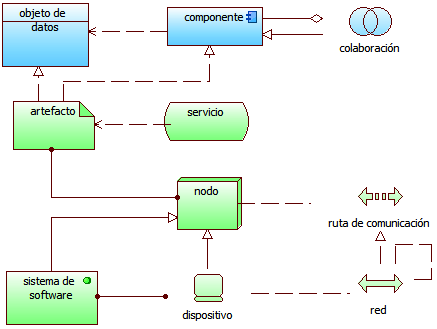
\includegraphics[scale=0.8]{figuras/13}
   	\captionsetup{width=.95\textwidth}
   	\caption{Interfaz Coloso}
   	\label{figura13}
  \end{figure}